\documentclass[14pt]{extbook}
\usepackage{multicol, enumerate, enumitem, hyperref, color, soul, setspace, parskip, fancyhdr} %General Packages
\usepackage{amssymb, amsthm, amsmath, bbm, latexsym, units, mathtools} %Math Packages
\everymath{\displaystyle} %All math in Display Style
% Packages with additional options
\usepackage[headsep=0.5cm,headheight=12pt, left=1 in,right= 1 in,top= 1 in,bottom= 1 in]{geometry}
\usepackage[usenames,dvipsnames]{xcolor}
\usepackage{dashrule}  % Package to use the command below to create lines between items
\newcommand{\litem}[1]{\item#1\hspace*{-1cm}\rule{\textwidth}{0.4pt}}
\pagestyle{fancy}
\lhead{Progress Quiz 4}
\chead{}
\rhead{Version C}
\lfoot{4378-7085}
\cfoot{}
\rfoot{Fall 2020}
\begin{document}

\begin{enumerate}
\litem{
Find the equation of the line described below. Write the linear equation as $ y=mx+b $ and choose the intervals that contain $m$ and $b$.\[ \text{Parallel to } 6 x - 7 y = 4 \text{ and passing through the point } (2, 8). \]\begin{enumerate}[label=\Alph*.]
\item \( m \in [0.8, 0.88] \hspace*{3mm} b \in [6.25, 6.43] \)
\item \( m \in [0.8, 0.88] \hspace*{3mm} b \in [-7.04, -6.05] \)
\item \( m \in [-1.62, -0.62] \hspace*{3mm} b \in [9.25, 10.45] \)
\item \( m \in [0.8, 0.88] \hspace*{3mm} b \in [5.56, 6.22] \)
\item \( m \in [1.05, 1.62] \hspace*{3mm} b \in [6.25, 6.43] \)

\end{enumerate} }
\litem{
First, find the equation of the line containing the two points below. Then, write the equation as $ y=mx+b $ and choose the intervals that contain $m$ and $b$.\[ (10, -8) \text{ and } (-6, -3) \]\begin{enumerate}[label=\Alph*.]
\item \( m \in [-0.61, -0.24] \hspace*{3mm} b \in [-19.8, -17.4] \)
\item \( m \in [-0.3, 0.37] \hspace*{3mm} b \in [-2, 2.5] \)
\item \( m \in [-0.61, -0.24] \hspace*{3mm} b \in [4.2, 5.5] \)
\item \( m \in [-0.61, -0.24] \hspace*{3mm} b \in [-5.7, -4.6] \)
\item \( m \in [-0.61, -0.24] \hspace*{3mm} b \in [-0.2, 4] \)

\end{enumerate} }
\litem{
Write the equation of the line in the graph below in Standard form $Ax+By=C$. Then, choose the intervals that contain $A, B, \text{ and } C$.
\begin{center}
    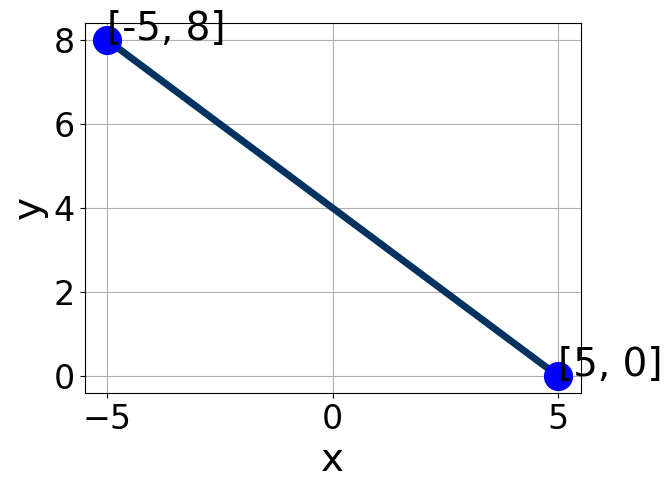
\includegraphics[width=0.5\textwidth]{../Figures/linearGraphToStandardC.png}
\end{center}
\begin{enumerate}[label=\Alph*.]
\item \( A \in [0.9, 4.1], \hspace{3mm} B \in [4.8, 5.1], \text{ and } \hspace{3mm} C \in [14, 17] \)
\item \( A \in [-4.4, -1.8], \hspace{3mm} B \in [-5.2, -3.5], \text{ and } \hspace{3mm} C \in [-15, -9] \)
\item \( A \in [-0.8, 1.3], \hspace{3mm} B \in [-1.6, -0.7], \text{ and } \hspace{3mm} C \in [-6, -2] \)
\item \( A \in [0.9, 4.1], \hspace{3mm} B \in [-5.2, -3.5], \text{ and } \hspace{3mm} C \in [-15, -9] \)
\item \( A \in [-0.8, 1.3], \hspace{3mm} B \in [-0.3, 1.8], \text{ and } \hspace{3mm} C \in [2, 5] \)

\end{enumerate} }
\litem{
First, find the equation of the line containing the two points below. Then, write the equation as $ y=mx+b $ and choose the intervals that contain $m$ and $b$.\[ (-11, 9) \text{ and } (-3, -2) \]\begin{enumerate}[label=\Alph*.]
\item \( m \in [-3.4, -0.1] \hspace*{3mm} b \in [-0.7, 1.6] \)
\item \( m \in [-0.9, 4.7] \hspace*{3mm} b \in [1.4, 4.4] \)
\item \( m \in [-3.4, -0.1] \hspace*{3mm} b \in [19.1, 21.1] \)
\item \( m \in [-3.4, -0.1] \hspace*{3mm} b \in [-6.7, -2.1] \)
\item \( m \in [-3.4, -0.1] \hspace*{3mm} b \in [6, 6.8] \)

\end{enumerate} }
\litem{
Solve the linear equation below. Then, choose the interval that contains the solution.\[ \frac{-4x -9}{4} - \frac{8x + 5}{7} = \frac{-4x + 4}{5} \]\begin{enumerate}[label=\Alph*.]
\item \( x \in [-1.28, 0.5] \)
\item \( x \in [-3.11, -1.84] \)
\item \( x \in [-13.75, -13.38] \)
\item \( x \in [-2.79, -1.42] \)
\item \( \text{There are no real solutions.} \)

\end{enumerate} }
\litem{
Solve the equation below. Then, choose the interval that contains the solution.\[ -4(12x -17) = -6(10x + 9) \]\begin{enumerate}[label=\Alph*.]
\item \( x \in [-10.5, -9.85] \)
\item \( x \in [-0.46, 0.83] \)
\item \( x \in [0.22, 1.43] \)
\item \( x \in [-1.41, -0.59] \)
\item \( \text{There are no real solutions.} \)

\end{enumerate} }
\litem{
Find the equation of the line described below. Write the linear equation as $ y=mx+b $ and choose the intervals that contain $m$ and $b$.\[ \text{Perpendicular to } 4 x + 9 y = 4 \text{ and passing through the point } (-10, 9). \]\begin{enumerate}[label=\Alph*.]
\item \( m \in [1.7, 3.5] \hspace*{3mm} b \in [31.5, 33.5] \)
\item \( m \in [1.7, 3.5] \hspace*{3mm} b \in [18, 25] \)
\item \( m \in [-3, -0.9] \hspace*{3mm} b \in [-17.5, -10.5] \)
\item \( m \in [1.7, 3.5] \hspace*{3mm} b \in [-34.5, -29.5] \)
\item \( m \in [-1.4, 1.1] \hspace*{3mm} b \in [31.5, 33.5] \)

\end{enumerate} }
\litem{
Solve the equation below. Then, choose the interval that contains the solution.\[ -11(-10x + 14) = -18(5x + 2) \]\begin{enumerate}[label=\Alph*.]
\item \( x \in [9.41, 9.62] \)
\item \( x \in [0.92, 1.59] \)
\item \( x \in [-1.27, -0.82] \)
\item \( x \in [0.59, 0.71] \)
\item \( \text{There are no real solutions.} \)

\end{enumerate} }
\litem{
Solve the linear equation below. Then, choose the interval that contains the solution.\[ \frac{-7x -7}{3} - \frac{-9x + 7}{6} = \frac{-6x -4}{7} \]\begin{enumerate}[label=\Alph*.]
\item \( x \in [418, 422] \)
\item \( x \in [-1.63, 2.37] \)
\item \( x \in [122, 126] \)
\item \( x \in [24, 27] \)
\item \( \text{There are no real solutions.} \)

\end{enumerate} }
\litem{
Write the equation of the line in the graph below in Standard form $Ax+By=C$. Then, choose the intervals that contain $A, B, \text{ and } C$.
\begin{center}
    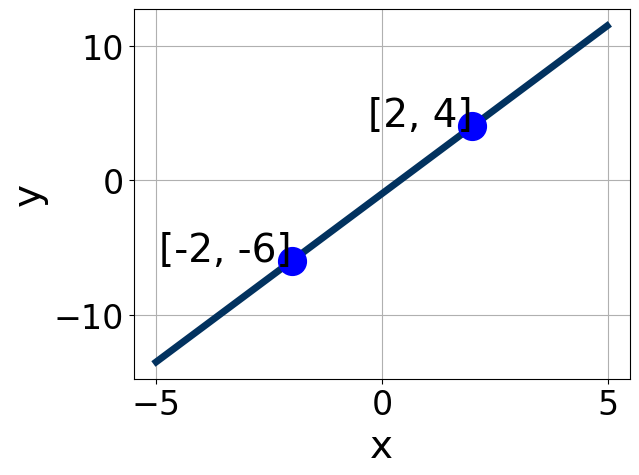
\includegraphics[width=0.5\textwidth]{../Figures/linearGraphToStandardCopyC.png}
\end{center}
\begin{enumerate}[label=\Alph*.]
\item \( A \in [-2.8, -1.8], \hspace{3mm} B \in [2.85, 3.32], \text{ and } \hspace{3mm} C \in [-6.2, -2.5] \)
\item \( A \in [-0.4, 5], \hspace{3mm} B \in [-3.88, -2.51], \text{ and } \hspace{3mm} C \in [1.7, 5.3] \)
\item \( A \in [-0.4, 5], \hspace{3mm} B \in [2.85, 3.32], \text{ and } \hspace{3mm} C \in [-6.2, -2.5] \)
\item \( A \in [-1.8, 1.6], \hspace{3mm} B \in [0.1, 1.66], \text{ and } \hspace{3mm} C \in [-1.6, -0.2] \)
\item \( A \in [-1.8, 1.6], \hspace{3mm} B \in [-2.63, 0.26], \text{ and } \hspace{3mm} C \in [-0.9, 2.1] \)

\end{enumerate} }
\end{enumerate}

\end{document}